\section{Project: Analyse blade grinder vibration}

\textbf{21022:} Here I'd like to talk a little about the difficulties encountered in the vibration analysis, such as my lack of knowledge of the subject, doubts about the reference system (local vs global),
the lack of real operational data and counter-intuitive results, and the need to strengthen the methodology and repeat the experiment

\todo{Improve existing Industrial production}

\subsection{Initial Hypothesis}
\paragraph{Client} Stumabo International, a manufacturer of precision blades for the food processing industry, produces several million blades per year and it is known in the industry for their progressive industrial potato cutting solutions,
and innovative shapes produced through hydro-cutting systems.
Stumabo also uses their knowledge to integrate the best blade in the FAM industrial mechanical cutters~\cite{Misc:stumabo_en_website}.

\paragraph{Context/Intro: Machine line}
\begin{figure}[ht]
    \begin{subfigure}{\textwidth}
        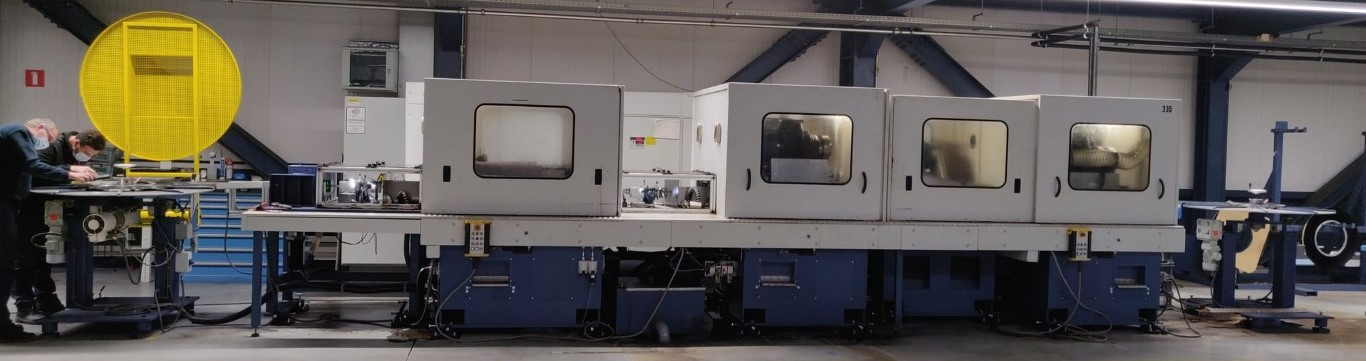
\includegraphics[width=\linewidth]{stumabo/installation/line_photo.jpg}
        \caption{Line overview: side view}
        \label{fig:line_overview}
    \end{subfigure}
    \begin{subfigure}{\textwidth}
        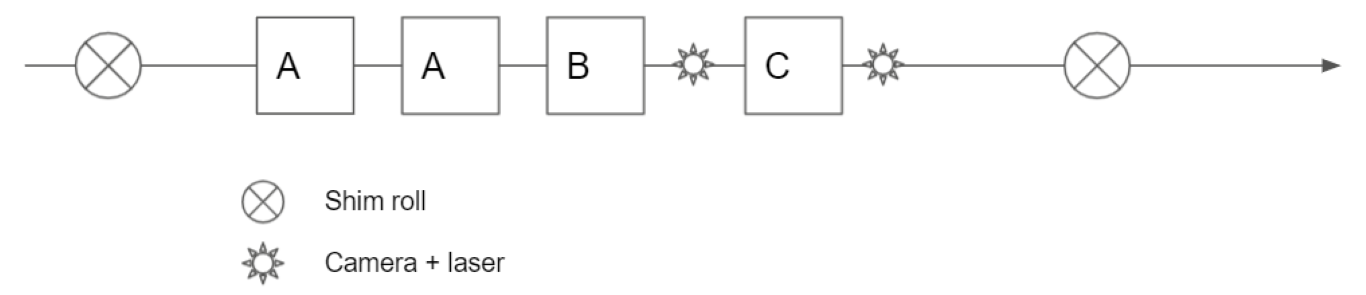
\includegraphics[width=\linewidth]{stumabo/installation/line_schematics.png}
        \caption{Line motor schematics}
        \label{fig:line_schematics}
    \end{subfigure}
    \caption{Stumabo's blade production line covered by this project}
    \label{fig:stumabo_prod_line}
\end{figure}

As shown in picture~\ref{fig:line_overview} there are four different stations with each one or two motors type ${A,B,C}$ (see figure: \ref{fig:line_schematics}).
Each station has grinding stones to sharpen a blade, which is one long strip of steel passing through all the machines.
To perform their grinding task, the stones turn around their axe sharpening the steel blade, each machine in its own way.

\subsection{Goal(s), purpose \& critical factors}
The project started in conjunction with the beginning of my internship experience (Oct-Nov 2021), and I had the pleasure of contributing in its early stages (\textit{ad-hoc} campaign);
\todo{DG: dare definizione di campagna ad hoc?}
unfortunately my practice ended before the second, more substantial phase of the project began (April 2022).
Let's see what the goals are in the long and short term and then exploring the latter.
\paragraph{Long Term: Project lifecycle}
\begin{itemize}
    \item[$\circledcirc$] Increase production quality through the use of continuos data analysis.
    \item[$\circledcirc$] Avoid unplanned standstill (downtime) by preventing critical components failure.
    \item[$\circledcirc$] Extends the life of machines and installation through \acl{PdM} and \acl{cm} (see Section \ref{section:maintenance})
\end{itemize}
\paragraph{Short Term: \textit{ad-hoc} campaign}
\begin{itemize}
    \item[$\circledcirc$] It is possible to identify a strong impact of the turning of the grindstones? Perhaps a possible imbalance?
    \item[$\circledcirc$] As a general insight, do we have indication that something is causing strong vibration?
    \item[$\circledcirc$] Lastly, as preliminary path for the \ac{CtM}, identify purpose.
\end{itemize}

\subsection{Project description by phases}
\begin{figure}[ht]
    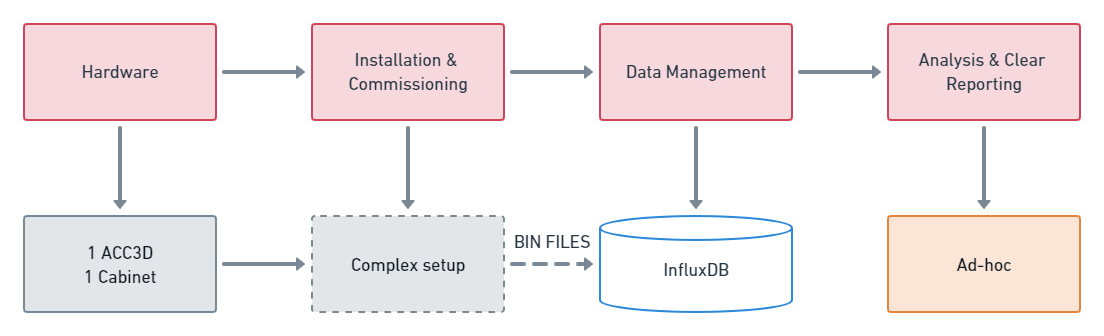
\includegraphics[width=\textwidth]{stumabo/21022_STU.png}
    \caption{Core Stages of this (full) project}
    \label{fig:stumabo_stages}
\end{figure}
As we saw together in section~\ref{section:zensor_approach}, we can have approximately two types of projects and this one a complete one.
However, as the reader will have already guessed, being a preparation campaign, as mentioned earlier, it will have less complexity than a big project.
My contribution was to help with the analysis phase, but it's important to emphasize how the first three phases went, because they will have serious implications for data development and analysis.

One 3-dimension accelerometer, called \textit{ACC3D} in \ref{fig:stumabo_stages}, and a ``mobile cabinet'' was provided to Stumabo, which they placed on each of the four machine and roughly kept track of the different positions and operations in a log file.
We must therefore clarify, before we go any further, the industrial setup; in our aid comes engineering schematics as shown in~\ref{fig:top_view and blade}.
\begin{figure}[ht]
    \begin{subfigure}{\textwidth}
        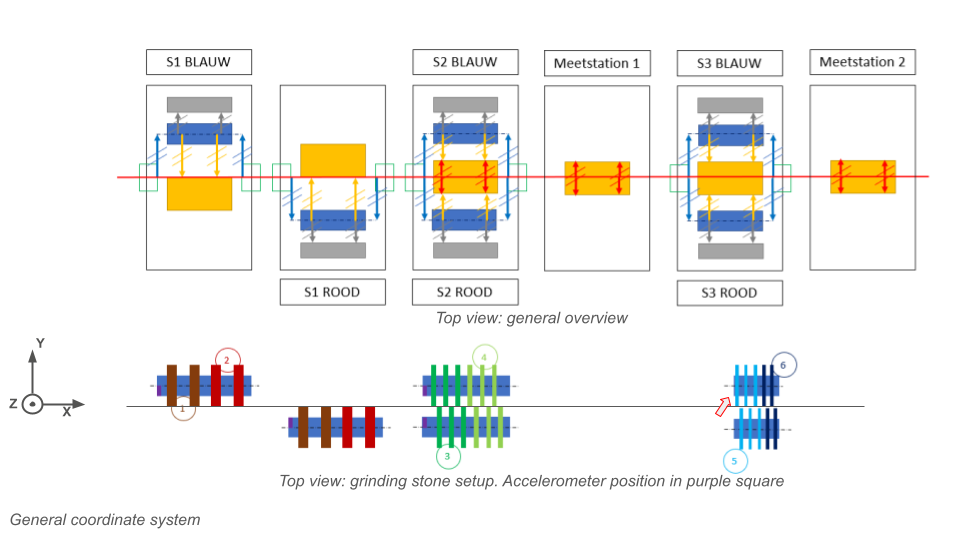
\includegraphics[width=.9\linewidth]{stumabo/installation/STU_General_Cordinate_System.png}
        \caption{Top view overview of stations plus grinding stones detail.
            Purple dots on the bottom details are where the ``ad-hoc'' accelerometer was placed}
        \label{fig:top_view_line}
    \end{subfigure}
    \begin{subfigure}{\textwidth}
        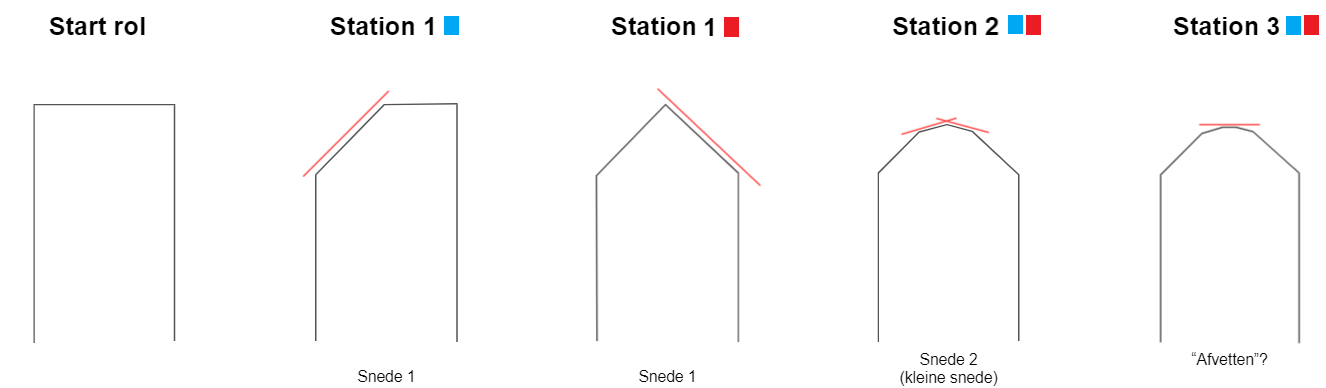
\includegraphics[width=.9\linewidth]{stumabo/installation/blade_processing.png}
        \caption{Blade evolution, a sketched overview of the cut by station}
        \label{fig:blade_evolution}
    \end{subfigure}
    \caption{Engineering schematic are important during analysis}
    \label{fig:top_view and blade}
\end{figure}

Thus, a single sensor was placed in different locations, remaining on for the duration of the ad hoc project. We will therefore have a single data stream.

%\subsection{Resources needed (to accomplish my task)}

% Before starting the actual monitoring campaign there has been an “ad-hoc” measurement campaign. One accelerometer + “mobile cabinet” *(the previous SST cabinet + ACC)* was provided to Stumabo, 
% which they placed on each machine and kept track of the different positions and operations in a log (Excel). RMS values were extracted by Damiano Gianotti and insights were derived by Yves (January 2022).

% A potential deeper investigation for the ad-hoc data is being proposed as of February 2022

% \begin{figure}[ht]
%     \begin{subfigure}{0.5\textwidth}
%         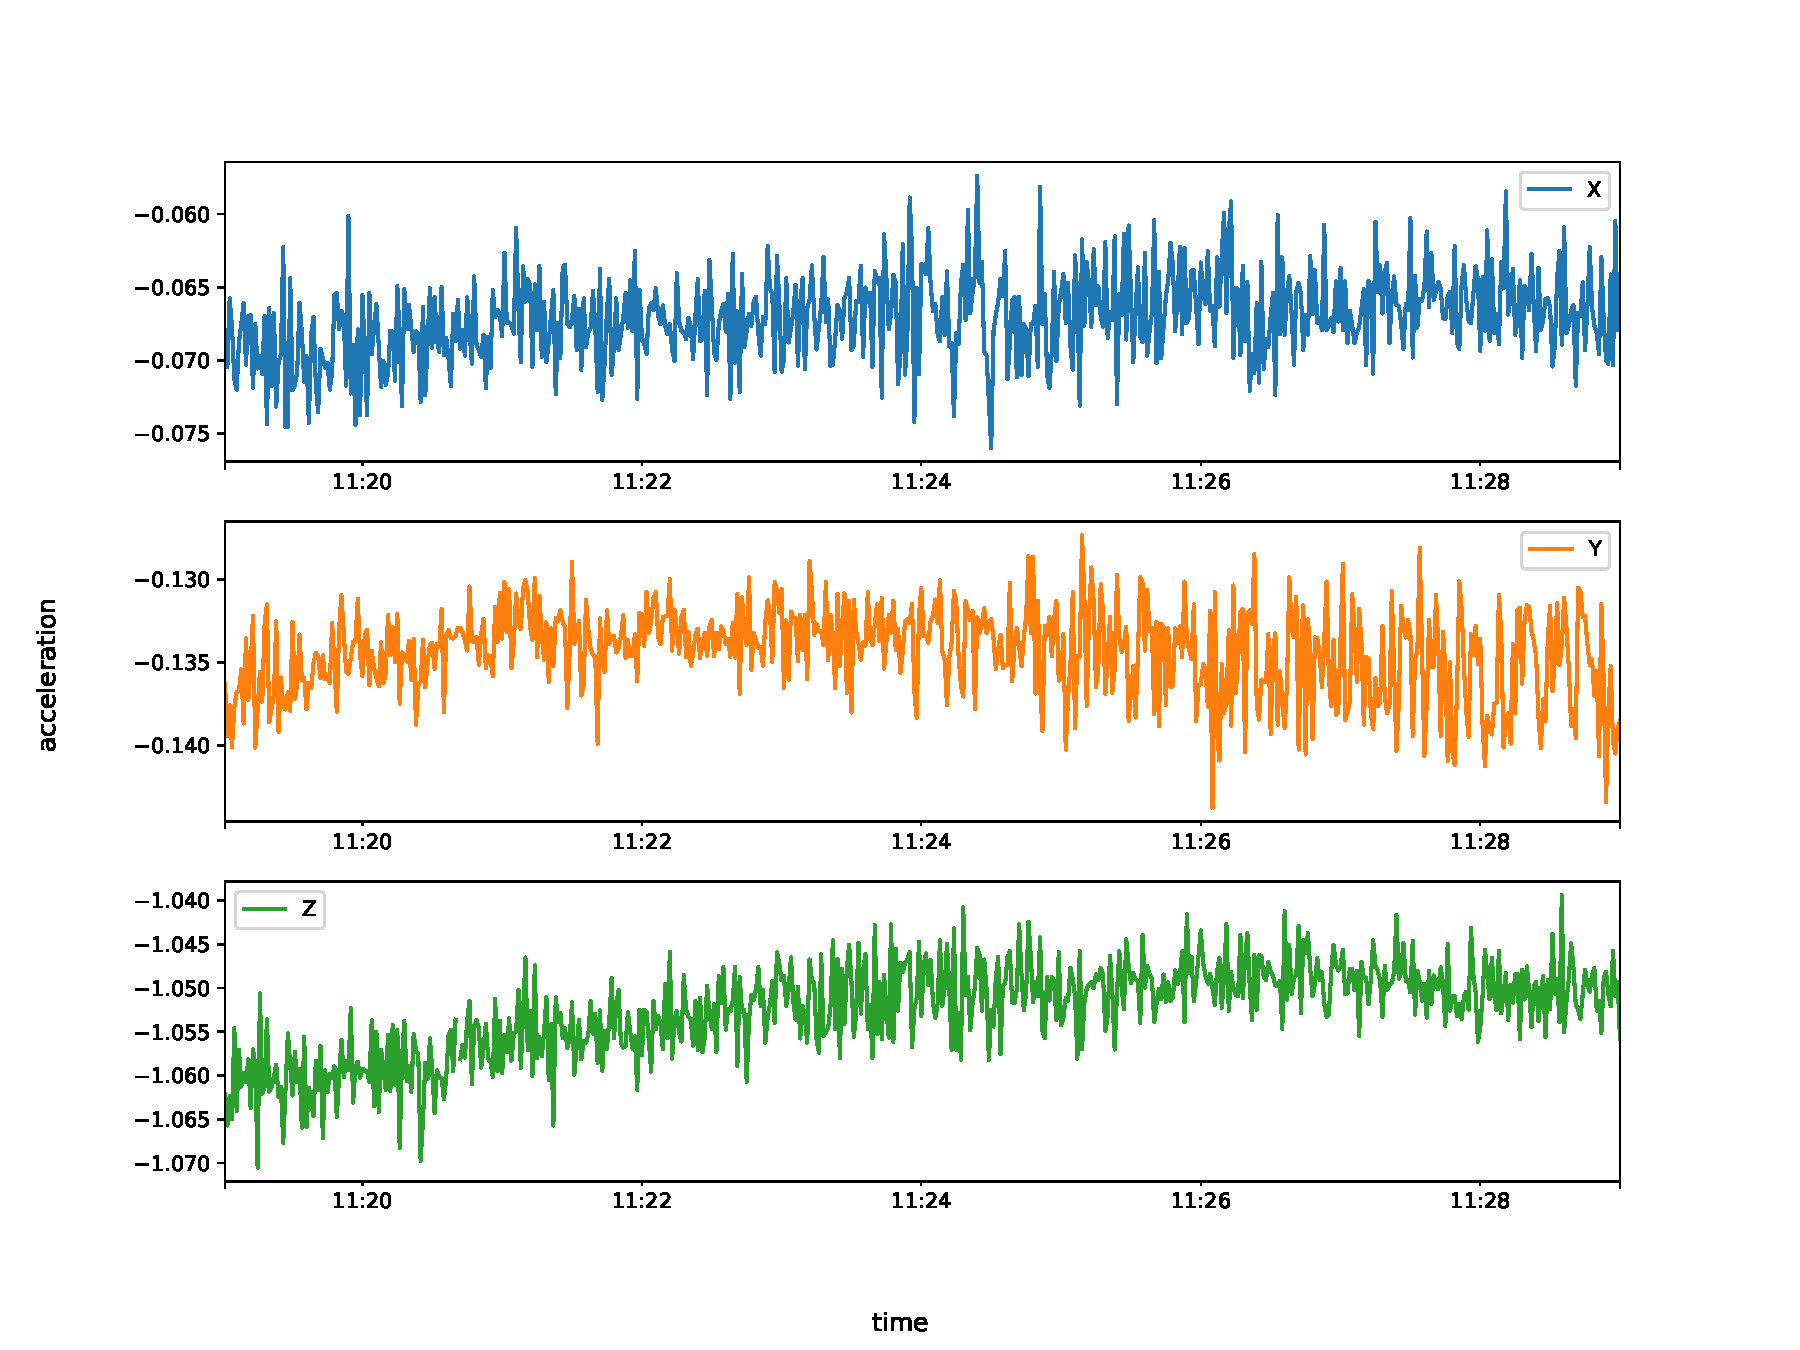
\includegraphics[width=\linewidth, height=6cm]{1hz-raw-vibration.pdf} 
%         \caption{Caption1}
%         \label{fig:subim1}
%     \end{subfigure}
%     \begin{subfigure}{0.5\textwidth}
%         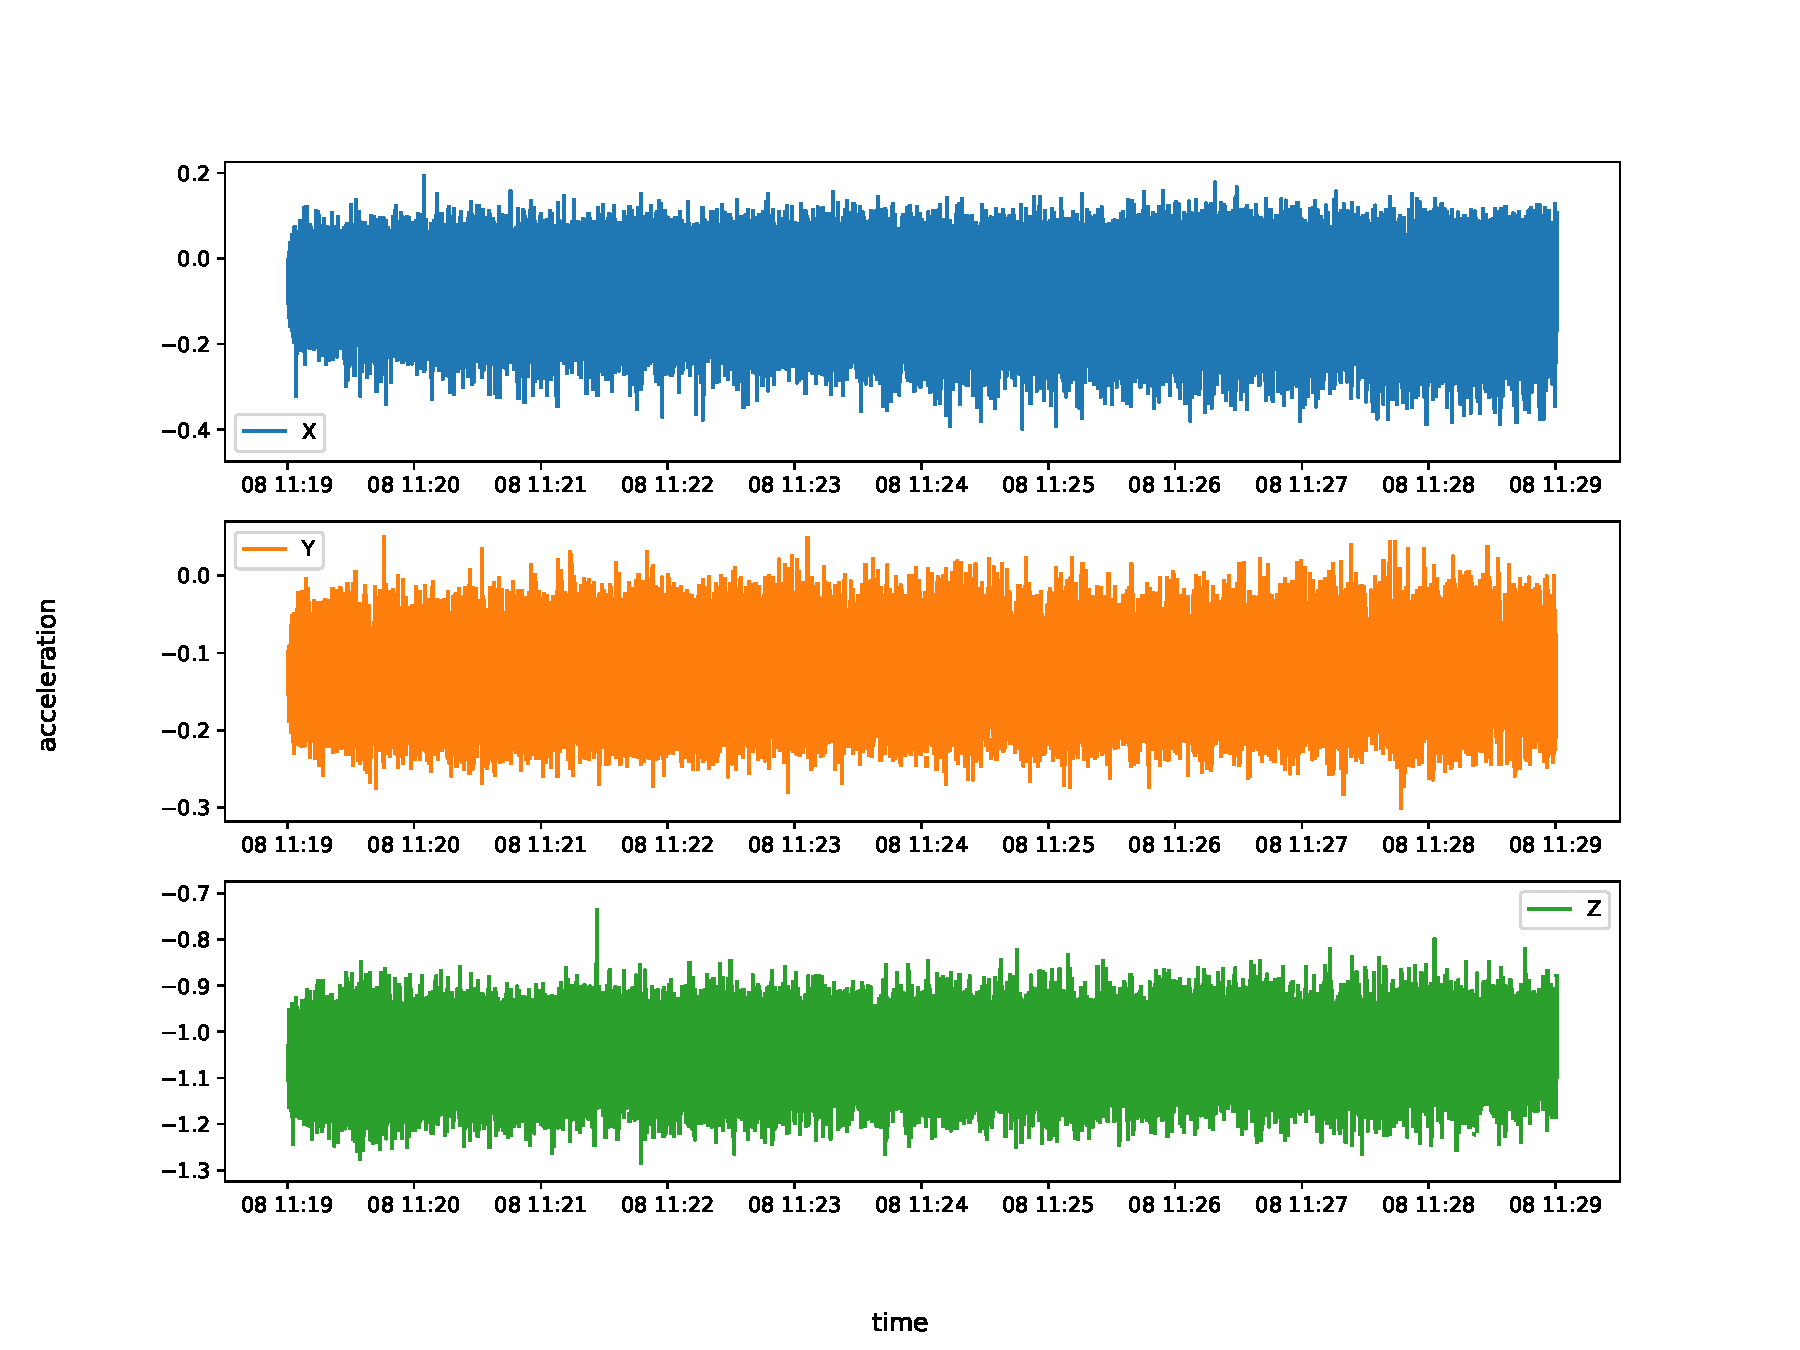
\includegraphics[width=\linewidth, height=6cm]{60hz-raw-vibration.pdf} 
%         \caption{Caption2}
%         \label{fig:subim2}
%     \end{subfigure}

%     \caption{Caption for this figure with two images}
%     \label{fig:image2}
% \end{figure}

% \begin{table}[h]
%     \centering
%     \begin{tabularx}{\textwidth}{@{}lllllllll@{}}
%     \toprule
%     start & einde & actie & kant & stat & draaien & $X$ & $Y$ & $Z$ \\ \midrule
%     13:19:01 & 13:29:01 & TEST & B & 1 & 1 & 131 & 176 & 592 \\ 
%     13:29:01 & 13:39:00 & TEST & B & 1 & 1,2 & 160 & 143 & 461 \\  
%     13:38:58 & 13:49:01 & TEST & B & 1 & 1,2,3B & 132 & 166 & 356 \\ 
%     13:48:59 & 13:59:00 & TEST & B & 1 & 1,2,3R & 113 & 149 & 244  \\
%     13:59:00 & 14:08:59 & TEST & B & 1 & 1,2,3B,3R & 145 & 143 & 217 \\ 
%     14:09:00 & 14:20:00 & TEST & B & 1 & 1,2,3B,3R,4 & 176 & 153 & 294 \\ 
%     \dots \\
%     10:04:00 & 12:35:00 & DASTE & B & 3 & 1,2,3B,3R,4 & 630 & 542 & 1489 \\
%     \bottomrule
%     \end{tabularx}
%     \caption{I valori vanno presi con $10^{-6}$}
%     \label{tab:my-table}
% \end{table}